\boste{What is the DDG? } \\ 
\boste{Why do we want a DDG?} \\
\boste{What properties should it have and why?} \\
The vertices $V$ in the dependency directed graph (DDG) $G=(V,A)$ initially only represent the variables and the 
constraints where the variable vertices only have outgoing arcs to the constraints they participate in. We want to 
change the CSOP model to a model more suited for local search, a CBLS model. The initial model will be modified by 
introducing invariants defined by oneway constraints and vertices representing invarints will be added to the graph 
$G$.  \\
The graph can be illustrated with all the variable vertices to the left and all constraint vertices to the right. 
Then the invariants vertices will be added in the middle. \\  
The invariants represents variables that are defined by oneway constraints or they can represent 
auxiliary variables used in the local search. If a variable is defined by a oneway constraint the variable vertex is 
removed from $G$ since we no longer changes the value of that variable directly. \boste{is it clear what that means? 
(directly)} \\ 
From now on when talking about vertices in $G$ it refers to the variable, invariant or constraint it represents unless 
other stated. \\
%The variables are non-fixed and non-defined and only have outgoing arcs. 
The vertex $v \in V$ has an outgoing arc to vertex $u \in V$ if and only if the value of $u$ is directly dependent on 
the value of $v$.
%Variables and invariants has an outgoing arc to the invariants that 
%depends on their value. \\ 
The DDG is needed in order to evaluate and update values of variables and invariants during local search. The graph 
$G$ is used to build the propagation queues described in subsection \ref{sec_propaqueue}. \\ 
It gets complicated to compute the propagation queues if there exist a strongly connected component in $G$. A 
\emph{strongly connected component} (scc) is a maximal set of vertices $V^{SCC}$ such that for each pair of vertices 
$(u,v) \in V^{SCC}$ there exist both a path from $u$ to $v$ and a path from $v$ to $u$ \cite[p. 1170]{cormen}. \\ 
Only invariant vertices can be part of a strongly connected component of size at least two, since variables vertices 
only have outgoing arcs and constraint vertices only have ingoing arcs. This indicates that there could be circular 
definition of variables. Because of this we want to avoid ending up with strongly connected components in the graph 
$G$. \medskip \\ 
This small example with three variables and a two constraint illustrates a possible graph $G$ and how invariants are 
introduced. 
\begin{center}
\begin{tabular}{rlr}
$ c_1: $&$2x_1 + x_2 - x_3 $&$= 2$ \\
$ c_2: $&$x_2 + x_3 $&$\leq 1$ \\
\end{tabular} 
\end{center}
Initially $G$ would consist of the three variables $x_1$, $x_2$, and $x_3$ and the constraints $c_1$ and $c_2$. The 
variable $x_3$ could be defined as an invariant $i_1$ by transforming $c_1$ to a oneway constraint. Once a 
variable is defined by a oneway constraint it is removed from the graph. Since $c_1$ is transformed it is removed from 
the $G$ and replaced by invariant $i_1$ which has ingoing arcs from $x_1$ and $x_2$. 

\begin{center}
    \begin{tikzpicture}[scale=1]
        \vertex[label=$x_1$](x1) at (0,2) {};
        \vertex[label=$x_2$](x2) at (0,0) {};
        \vertex[label=$i_1$](i1) at (2,1) {};
        \vertex[label=$c_2$](c2) at (4,0) {};

    \tikzset{EdgeStyle/.style={->}}
        \Edge(x1)(i1)
        \Edge(x2)(i1)
        \Edge(x2)(c2)
        \Edge(i1)(c2)
        %\Edge(y1)(c3)
        %\Edge(y2)(c3)
    \end{tikzpicture}
\end{center}
Auxiliary variable can be useful to speed up local search and in this example we could create an auxiliary 
variable $a_1$ which value is the sum of the left hand side of $c_2$. The auxiliary variable $a_1$ will be represented 
by an invariant $i_2$ which will be added to $G$. The invariant $i_1$, representing $x_3$, and variable $x_2$ have 
an outgoing arc to $i_2$ and $i_2$ have an outgoing arc to $c_2$. 


\begin{center}
    \begin{tikzpicture}[scale=1]
        \vertex[label=$x_1$](x1) at (0,2) {};
        \vertex[label=$x_2$](x2) at (0,0) {};
        \vertex[label=$i_1$](i1) at (2,1) {};
        \vertex[label=$i_2$](i2) at (4,0) {};
        \vertex[label=$c_2$](c2) at (6,0) {};

    \tikzset{EdgeStyle/.style={->}}
        \Edge(x1)(i1)
        \Edge(x2)(i1)
        \Edge(x2)(i2)
        \Edge(i1)(i2)
        \Edge(i2)(c2)

    \end{tikzpicture}
\end{center}
\boste{Talk about updating $x_2$}

%\end{minipage}
 
\boste{start on algorithms}
%The DDG $G$ is initially a bipartite graph where all the decision variables $X$ are vertices in one set and all the 
%constraints $C$ are vertices in the other set. If constraint $c$ applies to a variable $x$ then there is an arc from 
%the vertex representing $x$ to the vertex representing $c$. \\    
First all integer variables $Y$ in the CSOP $\mathbb{P}$ \boste{Should I call the models CSOP or just model?} get 
defined by oneway constraints by algorithm \ref{algo_makeints}. If some of the integer variables cannot be defined 
\boste{Currently report fail and exit}. 
\\
\IncMargin{1em}
\begin{algorithm}[H]
\SetKwData{Oneway}{oneway}
\SetKwFunction{makeIntVarOneway}{makeIntVarOneway}
\SetKwFunction{Next}{next}\SetKwFunction{Constraints}{Constraints}\SetKwFunction{Remove}{remove}
\SetKwFunction{intVarCanBeMadeOneway}{intVarCanBeMadeOneway}
\algdata 
\Input{A set $Y$ of integer variables sorted by decreasing domain size}
\Output{A CBLS model for local search}
\BlankLine
%\emph{special treatment of the first line}\;
\Bool $change = $ \true\;
\While{$Y \neq \emptyset$ \textbf{and} $change$}{
  $change = $\false \;
  \ForEach{$y_i \in Y$}{
    \upshape select \Var $y_i$ \upshape from $Y$\;
    \ForEach{\Con $c_j$ \upshape in $C(y_i)$}{
      \If{\intVarCanBeMadeOneway{$y_i$,$c_j$}}{
	\makeIntVarOneway{$y_i$,$c_j$}\;
	Remove $y_i$ from $Y$\;
	isOneway($c_j$) = \true \;
	$change = \true$\;
	\bre\;
      }
    }
  } \label{false}
}
\caption{Defining integer variables by one-way constraints}\label{algo_makeints}
\end{algorithm}\DecMargin{1em}
\noindent
For each of the variables $y_i$ each of the constraints $c_j$ that applies to $y_i$ is checked if it can be made oneway 
to define $y_i$ until one is found or none can be found. This is done until there are no integer variables left or the 
remaining integer variables cannot be defined, when the boolean change is false after line \ref{false}. Algorithm 
\ref{algo_checkintoneway} checks if constraint $c_j$ can be made oneway to define $y_i$ and algorithm 
\ref{algo_makeintoneway} transforms $c_j$ into a oneway constraint defining $y_i$ and updates the DDG $G$. \\
Let $\mathcal{F} = \{f_1,f_2,\dots ,f_k\}$ be the family of objective functions. \\
\IncMargin{1em}
\begin{algorithm}[H]

\SetKwFunction{relation}{relation}\SetKwFunction{coeff}{coefficient}
\SetKwFunction{objcoeff}{objectiveCoefficients}
\algdata
\Input{\Var $y_i$ and \Con $c_j$}
\Output{Boolean}
\BlankLine
\If{$c_j$ \upshape already defines a oneway constraint}{\Return{} \false\; \boste{This constraint could be removed in 
$O(\alpha(c_j))$}}

int $undefinedIntVar = 0$ \;
\ForEach{\Var $x$ \upshape in $c_j$}{
  \If{x is undefined integer variable}{
    $undefinedIntVar++$\;
  }
}
\If{$undefinedIntVar > 1$ \label{undefined}}{\Return{} \false  \boste{Insures no cycle is created} \; 
\tcp {else only $y_i$ is undefined integer variable}} 
%\If{$|Y(c)| > 1$}{\Return{} \false}
%\If{\relation{c} \upshape is (==) }{\Return{} \true}
\If{$c_j$ \upshape is linear equality}{\Return{} \true}
%\int coeff = \coeff{c,v}\;
%\upshape in $\bigcup\limits_{o \in O} f_o(\vec{v})$}{	
%\boste{The following is not at all correct, we should discuss this Tuesday} \\
\If{\upshape coefficient $c_{ij} \geq 0 $ \label{positivecoef}}{ 
  \Return{} \false \; 
}
\ForEach{ $f_j$  in $\mathcal{F}$ }{
  \If{$f_ij < 0$ \label{objectivecoef}}{
    \Return{} \false \;
    \boste{Not sure of to define coefficients in objective functions. coefficient of variable i in constraint j could 
be $c_{ij}$ but $c_j$ is used for constraint and then all variable $y_i$ should be $y_i$}
  }
}
\Return{} \true\;
 \caption{intVarCanBeMadeOneway( \textsf{Variable} $y_i$, \textsf{Constraint} $c_j$)} \label{algo_checkintoneway}
% \caption{Test if a constraint $c$ can define a variable $x$ } \label{algo_checkoneway}
\end{algorithm}
\DecMargin{1em}
If constraint $c_j$ already defines another variable it cannot be used to define $y_i$. Line \ref{undefined} makes sure 
that integer variable $y_i$ is not defining another integer variable $y_k$. This limits the model and increases the 
complexity of algorithm \ref{algo_makeints} because of the addition of the initial while loop. The 
condition in line \ref{undefined} makes sure that no strongly connected component of size 2 or greater is created in 
$G$. \boste{This should be described why we dont want that and what a SCC is}. The lines \ref{positivecoef} and 
\ref{objectivecoef} returns false if the coefficient of $y_i$ in $c_j$ is positive or one of the coefficients in the 
objective functions is negative. If that is not the case the constraint $c_j$ can define variable $y_i$ since we 
restrict the lower bound of $y_i$ by the oneway constraint and want to minimize its value in the objective functions. 
This gives some other complications which will be described after algorithm \ref{algo_makeintoneway}. \\ 
\IncMargin{1em}
\begin{algorithm}[H]
\algdata
\Input{\Var $y_i$ and \Con $c_j$}
\Output{Updated $G$}
\BlankLine
%\int $coef = A_{c,x}$\;
set $Q$ \tcp*[r]{new coefficient set}
set $U$ \tcp*[r]{new variable set}
\tcp{Move $y_i$ to right hand side and set coefficient to 1}
\ForEach{$x_k$ \upshape in $X(c_j)\setminus {y_i}$}{
  $c'_{kj} = -\frac{c'_{kj}}{c_{ij}}$ \;   
  $Q = Q\cup c'_{kj}$ \;
  $U = Q\cup x_k$ \;
}
%$Q = A_c \backslash \{A_{c,x}\}$\;
%$U = X(c) \backslash \{y_i\}$\;
%\ForEach{$A_{c,x}$ \upshape in $Q$}{
%  $Q_{c,x} = A(c,x) \cdot \frac{-1}{coef}$
%}
\tcp{Move right hand side to left hand side and update coefficient}
double $b' = \frac{B(c_j)}{c_{ij}}$ \;
\boste{coefficients can now be doubles (non integer)} \;
\If{$c_j$ \upshape is linear equality}{
  \textbf{invariant} $inv = $ new \Sum($U$,$Q$,$b'$)\;
  $G$ = $G \cup \{inv\}$\; 
  $G$ = $G \setminus \{c_j\}$\; 
  %\boste{Maybe remove $c$ from $G$}
  %\Return{\Sum{$V(c)$,$A(c)$,b}}
} \Else {
    \boste{Remember to say all constraints are either LQ or EQ} \;
    \textbf{invariant} $ inv= $ new \Sum($U$,$Q$,$b'$)\;
    \textbf{Invariant} $ inv' = $ new \Max{$inv$,lowerbound($y_i$)}\;
    $G$ = $G \cup inv$\; 
    $G$ = $G \cup inv'$\; 
    $G$ = $G \setminus \{c_j\}$\; 
% \boste{Maybe remove $c$ from $G$}
  %\Return{\Max{inv,b}}
}

 \caption{makeIntVarOneway(\textsf{Variable} $y_i$, \textsf{Constraint} $c_j$)} \label{algo_makeintoneway}
 %\caption{Make one-way constraint from $c$ defining variable $x$ } \label{algo_makeoneway}
 \end{algorithm}\DecMargin{1em} \noindent 
If the constraint $c_j$ is a linear equality constraint, an invariant $inv$ is defined by a new oneway constraint. The 
oneway constraint is made by isolating $y_i$ on the right side in $c_j$. Then $inv$ is added to $G$ and $c_j$ is 
removed from $G$. \\ 
If $c_j$ is not a linear equality constraint then it is a linear constraint with an upper bound $B(c_j)$. Since $c_ij$, 
the coefficient of $y_i$, in $c_j$ is negative $y_i$ can be isolated on the right hand side as an upper bound. The 
coefficients of $y_i$ in the objective functions are non-negative, know from algorithm \ref{algo_checkintoneway} line 
\ref{objectivecoef}. Variable    


Once all integer variables 
have been defined by oneway constraints, algorithm \ref{makefunc} is used to make each functional constraint into a 
oneway constraint defining a binary variable if possible. \\ 





Let $X$ be a set of variables and $x \in X$. The subset of constraints $C(x) \subseteq C$ is the set 
of constraints that applies to $x$.\\ 
The following algorithms describe how one-way constraints a create to define a variable $x$. \\ 



\IncMargin{1em}
\begin{algorithm}[H]
\SetKwData{Oneway}{oneway}

\SetKwFunction{makeOneway}{makeOneway}
\SetKwFunction{Next}{next}\SetKwFunction{Constraints}{Constraints}\SetKwFunction{Remove}{remove}
\SetKwFunction{canBeMadeOneway}{canBeMadeOneway}
\algdata 
\Input{A set $X$ of variables \boste{Sorting order?}}
\Output{A model better suited for local search}
\BlankLine
%\emph{special treatment of the first line}\;
\Bool $change = $ \true\;
\While{$X \neq \emptyset$ \textbf{and} $change$}{
  $change = $\false \;
  \ForEach{$x \in X$}{
    \upshape select \Var $x$ \upshape from $X$\;
    \ForEach{\Con $c$ \upshape in $C(x)$}{
      \Bool $flag = $ \canBeMadeOneway{c,x}\;  
      \If{$flag$}{
	\makeOneway{c,x}\;
	Remove $x$ from $X$\;
	$change = \true$\;
	\bre\;
      }
    }
  }
}
\caption{Defining integer variables by one-way constraints}\label{makefunc}
\end{algorithm}\DecMargin{1em}
\noindent
The algorithm tries to create invariants that define the set of variables $X$ by one-way constraints. It uses two other 
algorithms \canBeMadeOneway{c,x} and \makeOneway{c,x}. The first algorithm checks if the \cons $c$ can be used to define 
\var $x$ and the second algorithm transforms $c$ into a one-way constraint defining $x$. \\ 
The complexity of algorithm \ref{algo_defintvar} depends on the complexity of the two other algorithms but for 
simplicity let us assume they do not contribute for now. \\ 
Let $\alpha_{max}$ be the largest arity among all constraints in $C$ and $n$ be the number of decision variables in the 
input set. The size of $X$ has decrease by at least one each time we pass line 3 except for the first time. Hence line 3 
is passed at most $n$ times. Then the complexity of algorithm \ref{algo_defintvar} is $O(\alpha_{max} n^2)$. \\ \medskip
The coefficient of a variable $x_j$ in constraint $c_i$ is denoted $a_{ij}$. Let $\mathcal{F} = \{f_1,f_2,\dots ,f_k\}$ 
be the family of objective functions \boste{Think we should discuss this Tuesday} and the coefficient of variable $x_j$ 
in $f_k$ be $a_{kj}$. \boste{Maybe call it 
evaluation functions. Does not make sense since $a_{34}$ refers both to constraint and obj. func} \\  

\IncMargin{1em}
\begin{algorithm}[H]

\SetKwFunction{relation}{relation}\SetKwFunction{coeff}{coefficient}
\SetKwFunction{objcoeff}{objectiveCoefficients}
\algdata
\Input{\Con $c$ and \Var $x$}
\Output{Boolean}
\BlankLine
\If{c \upshape already defines a oneway constraint}{\Return{} \false\; \boste{This constraint could be removed in 
$O(\alpha(c))$}}
\If{\upshape Number of integer variables not defined $> 1$}{\Return{} \false\; \boste{Needed in order to create the 
right update queue}}
%\If{$|Y(c)| > 1$}{\Return{} \false}
\If{\relation{c} \upshape is (==) }{\Return{} \true}
%\int coeff = \coeff{c,v}\;
%\upshape in $\bigcup\limits_{o \in O} f_o(\vec{v})$}{	
\boste{The following is not at all correct, we should discuss this Tuesday} \\
\ForEach{a \upshape in $A(f(x))$ }{
  \If{$A(c,x) \cdot a > 0$}{
    \Return{} \false
  }
}
\Return{} \true\;
 \caption{canBeMadeOneway(\textsf{Constraint} c, \textsf{Variable} x)} \label{algo_checkoneway}
% \caption{Test if a constraint $c$ can define a variable $x$ } \label{algo_checkoneway}
\end{algorithm}
\DecMargin{1em}
\boste{Description not finished (done at all)}

%The variables that a constraint $c$ applies to is the scope $V(c)$. The constraints are of the type \class{Linear} and 
%a constraint $c$ have a right hand side $B(c)$. \\ 
\IncMargin{1em}
\begin{algorithm}[H]
\algdata
\Input{\Con $c$ and \Var $x$}
\Output{An Invariant}
\BlankLine
\int $coef = A_{c,x}$\;
$Q = A_c \backslash \{A_{c,x}\}$\;
$U = V(c) \backslash \{x\}$\;
\ForEach{$A_{c,x}$ \upshape in $Q$}{
  $Q_{c,x} = A(c,x) \cdot \frac{-1}{coef}$
}
\int $b = B(c)$ \;
\If{\relation{c} \upshape is (==) }{
  Invariant $c' = $ \Sum{$U$,$Q$,b}\;
  $G$ = $G \cup c'$\; 
  \boste{Maybe remove $c$ from $G$}
  %\Return{\Sum{$V(c)$,$A(c)$,b}}
}
\Else{
  Invariant $c' = $ \Sum{$U$,$Q$,b}\;
  Invariant $c'' = $ \Max{c',lb(x)}\;
  $G$ = $G \cup c'$\; 
  $G$ = $G \cup c''$\; 
  \boste{Maybe remove $c$ from $G$}
  %\Return{\Max{inv,b}}
}

 \caption{makeOneway(\textsf{Constraint} c, \textsf{Variable} x)} \label{algo_makeoneway}
 %\caption{Make one-way constraint from $c$ defining variable $x$ } \label{algo_makeoneway}
 \end{algorithm}\DecMargin{1em}
\boste{Description of algorithm here} \\
Consider the following three constraints as a small example. \boste{Should the example be introduced before the 
algorithms?}
\begin{center}
\begin{tabular}{rlr}
$ c_1: $&$2x_1 + y_2 -y_1 $&$= 2$ \\
$ c_2: $&$2x_1 - y_2 $&$= 2 $ \\ 
$ c_3: $&$x_1 +y_1 +y_2 $&$\leq 5 $
\end{tabular} 
\end{center}
At first $y_1$ cannot be defined by a \oneway but $y_2$ can be defined by $c_2$ and then $y_1$ can be defined by $c_1$. 
The order in which the \oneway are created matters. \boste{Not finished here, continue tomorrow morning} 
\begin{center}
    \begin{tikzpicture}[scale=1]
        \vertex[label=$x_1$](x1) at (-1,1) {};
        \vertex[label=$y_1$](y1) at (3,2) {};
        \vertex[label=$y_2$](y2) at (1,0) {};
        %\vertex[label=$c_3$](c3) at (5,1) {};
         %\vertex[label=$c_2$](c2) at (5,0) {};
    \tikzset{EdgeStyle/.style={->}}
        \Edge(x1)(y1)
        \Edge(y2)(y1)
        \Edge(x1)(y2)
        %\Edge(x1)(c3)
        %\Edge(y1)(c3)
        %\Edge(y2)(c3)
    \end{tikzpicture}
\end{center}

%algorithm \ref{algo_defintvar} first check if $y_1$ can be defined by a \oneway which it cannot since $c_1$ applies to 
%two integer variables. Then $y_2$ cannot be defined by $c_1$ but can be defined by $c_2$. Then $c_2$ is transformed 
%into a \oneway $c_2'$ that defines $y_2$ and it is added to the DDG $G$, $c_2: y_2 = 2x_2 -2$. T  


% \floatname{algorithm}{Finding One-way constraints}
%\begin{algorithm}[ht]
% \caption{O$(|V|^2C_{mav}$O$($\method{canBeMadeOneway()}$)$}
% \begin{algorithmic}\label{updateGraph1}
%  \STATE{$Q = \emptyset$}
%  \STATE{$V = $ model.getVariables()}
%  \STATE{V.sort()}
%  \STATE{\bool change = \true }
%  \WHILE{change}
%    \FOR{\var var in $V$}
%      \FOR{\cons cons in var.usedInConstriant()}
%	\IF{\method{canBeMadeOneway(var, cons)}}
%	  \STATE{V.remove(var)}
%	  \STATE{$Q.psuhback($var$)$}
%	  \STATE{\Break }
%	\ELSE
%	\STATE{change = \\false}
%	\ENDIF
%      \ENDFOR
%    \ENDFOR
%   % \STATE{laxer$++$}
%%{$j\leftarrow 1$ \TO $i-1$}
%  \ENDWHILE
% \end{algorithmic}
%
%\end{algorithm}


% \floatname{algorithm}{}
%\begin{algorithm}[ht]
% \caption{\bool \method{canBeMadeOneway}(\var \text{var}, \cons cons) \qquad O$(V_{mav} + $O$($\method{makeOneway}$))$}
% \begin{algorithmic}\label{updateGraph1}
% \IF{cons.isOneway()}
%  \RETURN \\false
%  \ENDIF
% \STATE{\Int notDefined = 0} 
% \FOR { \var v in cons.getVariables}
% \IF{v.isInteger()}
%  \IF{!v.isDefinedBxOneway}
%  \STATE{notDefined++}
%  \ENDIF
%  \ENDIF
%  \IF{notDefined $> 1$}
%    \RETURN \\false  
% \ENDIF
% \ENDFOR
% \STATE{\Int coef = var.getCoefficient(cons)}
% \STATE{\Int objCoef = var.getObjectiveCoefficient()}
% 
% \IF{cons.Relation = EQ \OR coef$\cdot$objCoef $< 0$}
%    \STATE{\method{makeOneway}(\var var, \cons cons)}
%    \RETURN \true
% \ENDIF
% \RETURN \\false
% \end{algorithmic}
%\end{algorithm}


% \floatname{algorithm}{}
%\begin{algorithm}[ht]
% \caption{\method{makeOneway}(\var \text{var}, \cons cons) \qquad O$(V_{mav})$}
% \begin{algorithmic}\label{updateGraph1}
% \STATE{variables = cons.getVariables()-var}
% \STATE{coefficients = cons.getCoefficient-var.coefficients}
% \STATE{\Int coef = var.getCoefficient(cons)}
% \IF{coef $\neq$ -1}
% \STATE{coefficients = $\frac{-1}{coef}\cdot$ coefficients}
% \ENDIF
% \STATE{\invar invar$(variables, coefficients)$}
% \FOR{\var v in variables}
%  \IF{v.isDefinedBxOneway}
%    \STATE{\invar inv = v.oneway}
%    \STATE{inv.updateList.pushback(invar)}
%  \ELSE
%  \STATE{v.updateList.pushback(invar)}
%  \ENDIF
%   \ENDFOR
%   \STATE{cons.isOneway = \true }
%   \STATE{cons.defines = invar }
%   \STATE{var.setDefinedBx(invar,cons)}
%   \STATE{model.add(invar)}
%   \STATE{invar.currentvalue = -cons.getArgument(1)} 
% \end{algorithmic}
%\end{algorithm}
  



